\documentclass[conference,10pt]{IEEEtran}
\IEEEoverridecommandlockouts
% The preceding line is only needed to identify funding in the first footnote. If that is unneeded, please comment it out.
\usepackage{cite}
\usepackage{amsmath,amssymb,amsfonts}
\usepackage{algorithmic}
\usepackage{graphicx}
\usepackage{textcomp}
\usepackage[T1]{fontenc}
\usepackage{mathptmx}
\def\BibTeX{{\rm B\kern-.05em{\sc i\kern-.025em b}\kern-.08em
		T\kern-.1667em\lower.7ex\hbox{E}\kern-.125emX}}
\begin{document}
	
	\title{Solving Multiplayer Snake using Competitive Self-play Reinforcement Learning}
	
	\author{\IEEEauthorblockN{Nitish Kumar Rath}
		\IEEEauthorblockA{\textit{University  of Florida}\\
			nitish.rath@ufl.edu}
		\and
		\IEEEauthorblockN{Sourav Dutta}
		\IEEEauthorblockA{\textit{University of Florida}\\
			duttasourav@ufl.edu}
		\and
		\IEEEauthorblockN{Srajan Paliwal}
		\IEEEauthorblockA{\textit{University of Florida}\\
			srajanpaliwal@ufl.edu}
	}
	
	\maketitle
	
	\begin{abstract}
		This project aims at solving one of the open research problems published by OpenAI\cite{n3}. This project is focused on implementing a multi-player clone of a Snake game based on the online hit \textit{slither.io}. The project aims to explore various reinforcement learning methodologies to solve the problem. This makes use of Gym toolkit by openAI as a base for reinforcement learning.
	\end{abstract}
	
	\begin{IEEEkeywords}
		deep learning, reinforcement learning
	\end{IEEEkeywords}
	
	\section{Introduction}
	Recently we have seen a rise in controlling agents using deep reinforcement learning directly from high-dimensional inputs. The inputs could be vision or speech or both combined. These are steps toward
	general artificial intelligence and these methods are directly applied to
	learn self play such as Alpha Go \cite{sp9} Atari \cite{sp3}. It has become
	evident that such algorithms achieve good performance on difficult problems
	without problem specific engineering. Also, it has been observed that the
	strategies are more complex than the environment. With traditional RL the
	rewards for a step were immediately available, but with games there can be
	complex strategies as the rewards can be a result of several consecutive steps.
	These methods use a wide variety of techniques like Markov decision process,
	discounted future reward, Q-learning \cite{sd5} and Policy gradient \cite{sd4}.\break
	This proposal aims at solving a multi-player snake game proposed by OpenAI as a open research topic and inspired by
	\textit{slither.io} \cite{sd2} where snakes consume food to increase length and
	kills other snakes. The game will be developed as a
	OpenAI Gym \cite{sd2} environment which provides an interface between the game
	and the learning algorithm. It allows developers to focus on the learning
	environment with much less stress on interacting with the game.
	
	\section{Related Work}
	Watkins\cite{sp1} introduced Q- learning as a simple way for training agents to learn
	optimal policies for a Markov decision process. Then, Tan\cite{sp2} further extend
	this idea to multiagents, his paper demonstrated that
	multi-agents can learn cooperative behavior in a simulated social environment with reinforcement learning.
	
	In past couple of years, a combination of deep neural network, Q-learning and
	competitive self play has allowed researchers to train agents for a variety
	of complex tasks. DeepMind\cite{sp3} used CNN and Q-learning to train deep Q-neural
	network agent that achieved scores comparable to professional human game
	testers in 49 Atari games. This was the first example of an AI algorithm
	that can excel at different tasks. DeepMind further improved DQN by introducing
	techniques like Double Q Learning\cite{sp4}, Prioritized Replay\cite{sp5}, Dueling DQN\cite{sp6}.  After
	that, Deep mind made a Go-bot\cite{sp7} based on a combination of deep Q-neural
	networks and tree search. It plays like a human player and can be compared to the top players. Neural networks were trained by supervised and reinforcement learning using human
	expert moves. The tree search algorithm
	combined neural network evaluations with Monte Carlo rollouts. In 2017, Alpha
	Go zero\cite{sp8} introduced an algorithm that learns without any human inputs.
	This algorithm learns through reinforcement self-play from scratch i.e. it starts
	with random plays and keeps improving itself. The search algorithms to evaluate moves used a single
	neural network without Monte Carlo rollouts.
	
	OpenAI experimented with competitive and cooperative self-play\cite{sp9}. They simulated
	multiple 3D-multiagent environments and demonstrated that agents can learn
	complex skills in simple environments with simple rewards. OpenAI\cite{sp10} used
	self-play to create a Dota 2 bot that defeated professional players in a
	constrained 1v1 match.
	\break
	\break
	Tampuu, Matiisen et al\cite{sd7} explored multi-agent environments and observed how the agents performed based on the reward system. They performed the experiments on Pong game. The most interesting experiment which is relevant to our project is simulating a collaborative and competitive environment and observe how agents interact. In the work done by Tampuu, Matiisen et al\cite{sd3}, the player was rewarded when the opponent lost in a competitive environment, whereas in a collaborative environment both players we penalized when any one of them lost. They clearly observed different agent behavior for these cases.
	\break
	\break
	We would like to experiment this on a multi-agent snake game where the snakes can be rewarded not only on the amount of food consumed but how many snakes are alive at any given moment. In a collaborative environment the snakes should avoid killing other snakes and avoid death to consume the available food. However, in a competitive environment a snake should focus on how it is able to stay alive longer and consume more food.
	
	
	\section{System Architecture}
	\begin{figure*}[]
		
		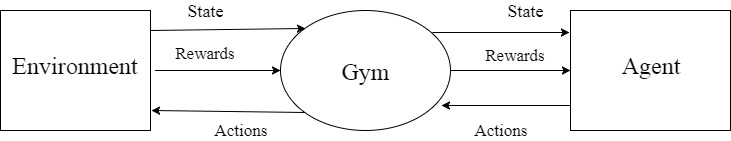
\includegraphics[width=\linewidth]{flow.jpg}
		\caption{Rough Flow of the algorithm}
		\label{test}
		
	\end{figure*}
	\begin{figure}[]
		
		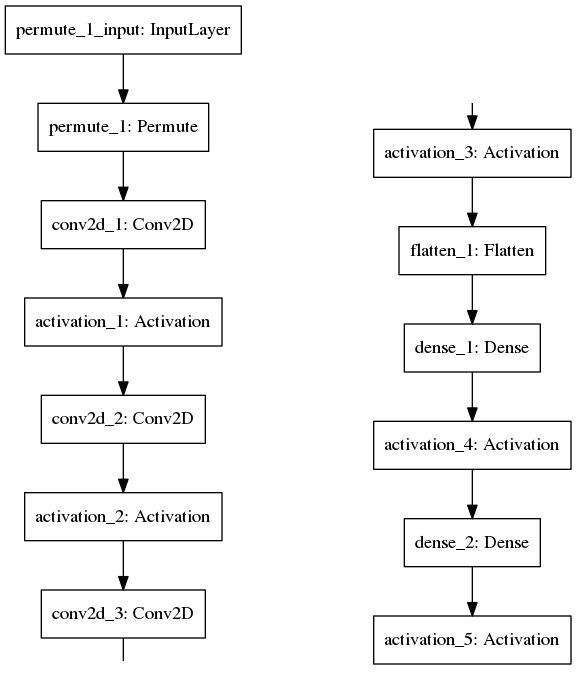
\includegraphics[scale=0.5]{model.png}
		\caption{Network Model}
		\label{model}
		
	\end{figure}
	Our system consists of three major components: Interface, Environment and Agent, with Interface acting as the bridge between the game(Environment) and Agent(algorithm).
	
	\subsection{Interface}
	We are using OpenAI Gym\cite{sd3} as an Interface between the game and the training agent. OpenAI Gym provides APIs to interact with the game environment. It is a toolkit for developing and comparing reinforcement learning algorithms and provides some pre-built game environments to experiment with. For these games we can focus primarily on the algorithm and not worry about how the game works. Interactions with the game include initializing a game, ending or resetting the ongoing game and stepping through the game. The step function takes one action from a pre-defined set of actions called "action space". On completion of the step function, an "observation space" is returned. The observation space contains the game state after an action has been performed and varies from game to game. It can be as simple as the current game snapshot  or any complex data like coordinates and speed of each entity in the game. It also contains a reward for the current action taken and a flag which states whether the game ended or not.
	\subsection{Environment}
	The environment is the game that the agent tries to learn. Our first requirement was to build a snake game compatible with OpenAI Gym APIs. One of the snake game implementations which was similar to what we required was implemented by Loonride\cite{sd4}. We modified the game and added a layer on top of it to act as wrapper and make it compatible with Gym. The game was built in JavaScript using Phaser game engine. For the ease of use and make minimal changes we simulated the browser experience in a headless mode using selenium web driver. 
	\break
	\break
	We modified the game to expose information like coordinates of the snakes, scores, whether the snakes is alive or not, food positions and the current game snapshot. This information is used by the agent algorithm to learn the game play. Furthermore, the input to the snake bot was also changed to take inputs from the action space instead of input devices such as mouse or keyboard.
	\break
	Upon training it was discovered that the process was too slow due to communication latencies in the selenium driver. Therefore, we moved to a simpler game environement, although this was a more realistic environment.The python game uses PyGame and is much faster than the JavaScript versoin. The snake in this case has less degrees of freedom. It can go either forward or turn left or right. It is a pixelated game where the entire game space can be consired as nxn blocks or big pixels and the snake can move one block at a time. Similarly the food is of size 1x1 block. We have two versions of the game. First, there is only one food and a new food appears randomly on the screen when it is consumed. In the second version there are more than one food. This game also runs on server in a headless or non-ui mode.
	
	
	\subsection{Agent}
	The agent here is the algorithm that runs the players in the game. In our work we chose to use Q-learning, a form of reinforcement learning to figure out the game play by using the feedback provided by the game. Our training algorithm was inspired by Deep Q-learning technique proposed by DeepMind\cite{n4}.
	\break
	\break
	We made use of the Keras implementation of the Deep Q-learning developed by Matthias Plappert.\cite{n5}. This library also contains some other implementation of reinforcement algorithms like Double DQN and SARSA. It works with tensorflow backend and can be trained on a CPU and GPU and is also compatible with the APIs of OpenAI Gym.
	\break
	\break
	We made use of the network as proposed by DeepMind as a agent. Our network receives the game state and decides on a action. It then uses the feedback, rewards and observation pertaining to the action, from the game to backpropagate and approximates a Q-function for efficient game play.
	Figure\ref{model} shows the model that we implemented
	
	\section{Algorithms}
	Our work makes use of reinforcement learning, Q-learning to be specific to observe the game and approximate a appropriate function for game play. The following give details about the algorithm and policies used to train it.
	
	\subsection{Q-Learning}
	Q- learning is a reinforcement learning technique where a function Q(s,a), where is the s is the present state and a is the action to be performed, is learnt to produce efficient actions for a given state s. The function is highly environment dependent and varies with every environment. In simple words it gives the optimal score that can be gained in the current state so that the overall game score is maximum at the end of it. This means that the function must take in account the possible future rewards to determine an efficient action. To accomplish this, it must be aware of the rewards of all <s,a> pairs. In simple game environment like tic-tac-toe, all <s,a> pairs can be listed in a table and Q-values updated to converge at a optimum point. In scenarios like atari games or Snake, the number of <s,a> pairs is too large to record. Also most of this may never be visited. Hence, DeepMind came up with a modified Q-learning technique, \textit{Deep Q-Networks}, based on Deep learning to efficiently approximate the Q-function.
	
	\subsection{Exploration-Exploitation Dilemma}
	As discussed above, it is difficult to map all <s,a> pairs in complex game environments. There is always a dilemma between choosing a new action for a state to explore new states or going on with the previous learned actions to exploit more from the game play. Thus there has to be a effective trade-off between the two for learning the game optimally. DeepMind came up with policies to deal with this. Our work implements them and gives a comparative result.
	\break
	\break
	One such policy is \( \epsilon \)GreedyPolicy . This is a improvement on greedily choosing a know <s,a> pair. In this the algorithm may choose to take a new action based on a probability defined by  \( \epsilon \). The algorithm chooses to take a action inorder to exploit the game but may choose to take a explorative action the game depending on the probability.
	\break
	\break
	Another such policy is BoltzmannQpolicy, which is purely explorative. The policy chooses to takes an action based on the probability according to the predicted Q values. 
	\break
	\break
	Usually, in practice, a explorative policy is chosen during training and a exploitative policy is chosen during testing.

	
	\section{Results And Discussion}
	\begin{figure}[]
		
		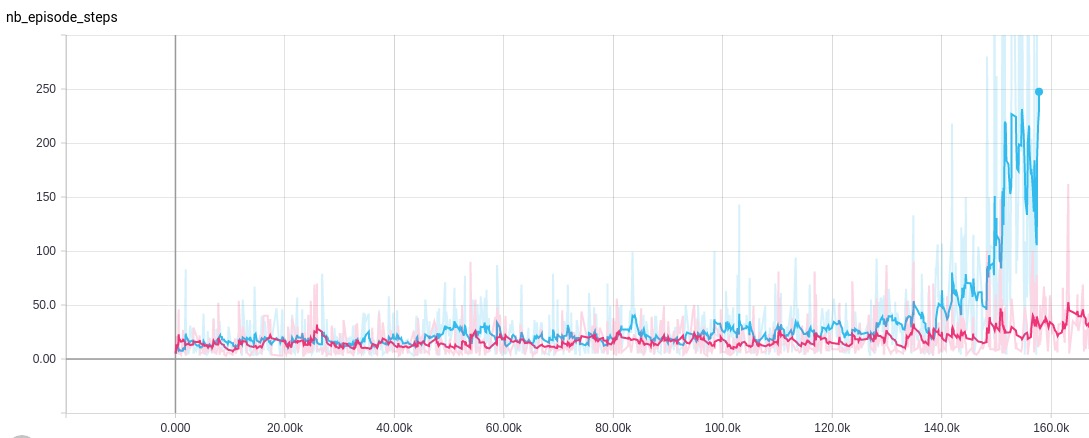
\includegraphics[scale=0.23]{ep_step.jpeg}
		\caption{Number of steps per Episode}
		\label{step}
		
	\end{figure}
	\begin{figure}[]
		
		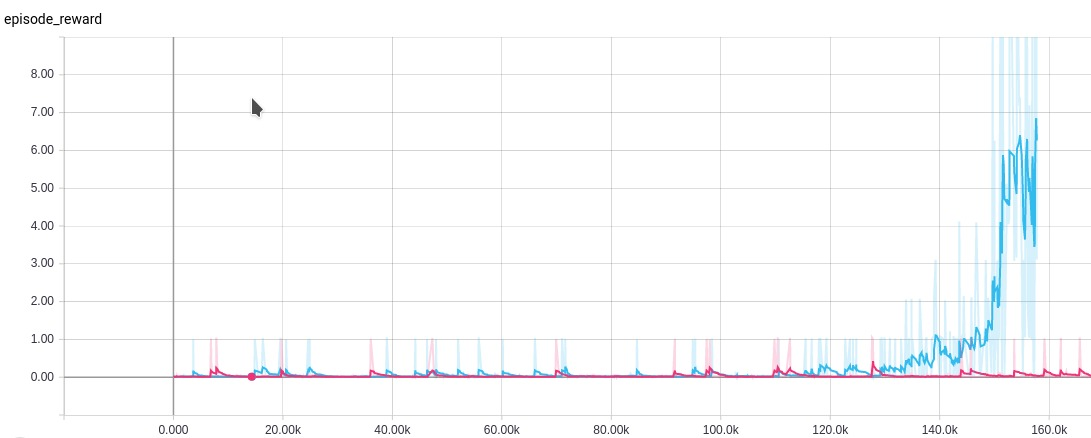
\includegraphics[scale=0.23]{ep_reward.jpeg}
		\caption{Rewards per episode}
		\label{reward}
		
	\end{figure}
	\subsection{Experimental Setup}
	The algorithms and the game environment were coded using python (using Keras and pygame libraries). The code was downloaded into a azure server and executed on it after setting up required configurations. We used a standard NC6 azure server with Nvidia K80 GPUs. The server run on linux. 
	\break
	\break
	The algorithm were run for 1.5 million steps and the reward and other logs were recorded.We saved weights for our agents at every 25,000 steps. This was done to analyze agent performance at various stages of learning. 
	\subsection{Results}
	
	Logs for the execution were monitored using Tensorboard library. Tensorboard is developed as a wrapper for Tensorflow and works with Keras library for monitoring performance of the training process.
	\break
	\break
	As can be seen from Fig.\ref{step} as the number of steps in training continued the reward obtained after each step also increased significantly. The blue plot in the figure is for the training with \(\epsilon\)GreedyPolicy and the pink one corresponds to the training with BoltzmannQpolicy. 
	\break
	\break
	Figure.\ref{reward} shows that the number of steps per episode increases with training. This implies that as the training continues the snake is learning to stay alive for a longer durations than before. 
	
	\subsection{Observations}
	We would like to discuss some interesting patterns that we observed the agent learning. Initially, an agent acts randomly and most of the games end by the agent hitting itself. By 125 thousand steps, the agent learns to avoid hitting itself and moves mostly in a straight line. At this point, most games end by agent hitting the boundary wall. By 325 thousand steps,  the agent learns to avoid hitting the wall by just moving in a loop. This is a good temporary strategy, but the agent is not receiving a significant reward. So in just 50 thousand steps more, it learns to break out of the loop and chase foods. The game length is short at this point due to collisions with walls and itself in attempt to eat food. The overall performance further improves as we give our agent more time to train.

\section{Future Work}
As of now, our team has successfully implemented a single player snake game environment, implemented a DQN learning algorithm for training it and has also run mltiple training iterations to fine tune the game play.
\break
\break

We have also started working on the multi player version of the game. The game environment is up and running and we have implemented a simple DQN learning algorithm for it by initiating multiple networks and training them separately on each agent by the rewards each agent receives from the game.
The training for it seems to take a lot of time. A possible reason for this may be due to the sequential pattern of training (each agent gets trained sequentially one after the other durig BackProp). We plan to eliminate this by exploring python threads and implementing them efficiently with Tensorflow.
\break
\break
\subsection{Task Completion Percentages}
\begin{itemize}
\item{Create a sigle Player Environment for snake Game} : 100\%	done
\item{Develop a training algorithm for Single Player Game play} :100\% done
\item{Create a Multi Player Environment for snake Game} : 100\%	done
\item{Develop a training algorithm for Multi Player Game play} :40\% done
\item{Explore other network architectures for GamePlay} :0\% done
\end{itemize}

\break
\break
In addition to fine tuning the multi player game, we also hav plans to explore other architectures to see if the training can be made better and the game play improved.
\break
\break


\begin{thebibliography}{00}
\bibitem{sp1} Watkins, C.J. and Dayan, P., 1992. Q-learning. Machine learning, 8(3-4), pp.279-292.
\bibitem{sp2} Tan, M., 1993. Multi-agent reinforcement learning: Independent vs. cooperative agents. In Proceedings of the tenth international conference on machine learning (pp. 330-337).
\bibitem{sp3} Mnih, V., Kavukcuoglu, K., Silver, D., Graves, A., Antonoglou, I., Wierstra, D. and Riedmiller, M., 2013. Playing atari with deep reinforcement learning. arXiv preprint arXiv:1312.5602.
\bibitem{sp4} Van Hasselt, H., Guez, A. and Silver, D., 2016, February. Deep Reinforcement Learning with Double Q-Learning. In AAAI (Vol. 16, pp. 2094-2100).
\bibitem{sp5} Schaul, T., Quan, J., Antonoglou, I. and Silver, D., 2015. Prioritized experience replay. arXiv preprint arXiv:1511.05952.
\bibitem{sp6} Wang, Z., Schaul, T., Hessel, M., Van Hasselt, H., Lanctot, M. and De Freitas, N., 2015. Dueling network architectures for deep reinforcement learning. arXiv preprint arXiv:1511.06581.
\bibitem{sp7} Silver, D., Huang, A., Maddison, C.J., Guez, A., Sifre, L., Van Den Driessche, G., Schrittwieser, J., Antonoglou, I., Panneershelvam, V., Lanctot, M. and Dieleman, S., 2016. Mastering the game of Go with deep neural networks and tree search. nature, 529(7587), pp.484-489.
\bibitem{sp8} Silver, D., Schrittwieser, J., Simonyan, K., Antonoglou, I., Huang, A., Guez, A., Hubert, T., Baker, L., Lai, M., Bolton, A. and Chen, Y., 2017. Mastering the game of go without human knowledge. Nature, 550(7676), p.354.
\bibitem{sp9} Bansal, T., Pachocki, J., Sidor, S., Sutskever, I. and Mordatch, I., 2017. Emergent complexity via multi-agent competition. arXiv preprint arXiv:1710.03748.
\bibitem{sd5} Qicheng Ma, Hadon Nash, ``Solving Multiplayer Games with Reinforcement Learning,".
\bibitem{sd1} G. Brockman, V. Cheung, L. Pettersson, J. Schneider, J. Schulman, J. Tang, and W. Zaremba. OpenAI Gym. arXiv preprint arXiv:1606.01540, 2016.
\bibitem{sp10} OpenAI. (August 2017). Dota 2. [online] Available at: https://blog.openai.com/dota-2/ [Accessed 1 Feb. 2018].
\bibitem{sd2} Slither.io [online] Available at: http://slither.io/ [Accessed 1 Feb. 2018].
\bibitem{sd3}https://github.com/openai/gym
\bibitem{sd4}https://github.com/Loonride/slither.io-clone
\bibitem{n2} TensorFlow [online] Available at: https://www.tensorflow.org [Accessed 1 Feb. 2018].
\bibitem{n3} OpenAI Blog [online] Available at: https://blog.openai.com/requests-for-research-2/ [Accessed 1 Feb. 2018].
\bibitem{n4}https://arxiv.org/abs/1312.5602
\bibitem{n5}https://github.com/keras-rl/keras-rl
\bibitem{sd7}Ardi Tampuu, Tambet Matiisen, Dorian Kodelja, Ilya Kuzovkin, Kristjan Korjus, Juhan Aru, Jaan Aru, Raul Vicente, ``Multiagent Cooperation and Competition with Deep Reinforcement Learning".
\end{thebibliography}

\end{document}
